\subsection{Cosmic Radiation Results}
\label{sec:Cosmic-Radiation-Results}

This is the cosmic radiation results.

\begin{figure}[h!]
\hfill
\subfigure[MiniPIX counts measured during flight.]{\includegraphics[width=8cm]{figures/mp_counts.pdf}}
\hfill
\subfigure[MiniPIX dose measure during flight.]{\includegraphics[width=8cm]{figures/mp_dose.pdf}}
\hfill
\caption{MiniPIX particle data detected during flight.}
\label{minipix-data}
\end{figure}

\begin{figure}[h!]
\hfill
\subfigure[FITPix counts measured during flight.]{\includegraphics[width=8cm]{figures/fp_counts.pdf}}
\hfill
\subfigure[FITPix dose measure during flight.]{\includegraphics[width=8cm]{figures/fp_dose.pdf}}
\hfill
\caption{MiniPIX particle data detected during flight.}
\label{minipix-data}
\end{figure}

\begin{figure}[h!]
\subfigure[Histogram of the LET from each cluster type collected by the MiniPIX during flight.]{\includegraphics[width=12cm]{figures/mp_track_let_histogram.pdf}}
\hfill
\subfigure[Density plot of the LET from each cluster type collected by the MiniPIX during flight.]{\includegraphics[width=12cm]{figures/mp_track_let_density.pdf}}
\hfill
\caption{MiniPIX LET distributions from flight data.}
\label{fig:minipix-let}
\end{figure}

\begin{figure}[h!]
\subfigure[Histogram of the LET from each cluster type collected by the FITPix during flight.A logarithmic scale was used for the y-axis due to the small blob counts being relatively larger than all other counts.]{\includegraphics[width=12cm]{figures/fp_track_let_histogram.pdf}}
\hfill
\subfigure[Density plot of the LET from each cluster type collected by the FITPix during flight.]{\includegraphics[width=12cm]{figures/fp_track_let_density.pdf}}
\hfill
\caption{FITPix LET distributions from flight data.}
\label{fig:fitpix-let}
\end{figure}



\begin{figure}[h!]
\subfigure[Data from photodiode 0.]{\includegraphics[width=8cm]{figures/photo_0.pdf}}
\hfill
\subfigure[Data from photodiode 1.]{\includegraphics[width=8cm]{figures/photo_1.pdf}}
\hfill
\subfigure[Data from photodiode 2.]{\includegraphics[width=8cm]{figures/photo_2.pdf}}
\hfill
\subfigure[Data from photodiode 3.]{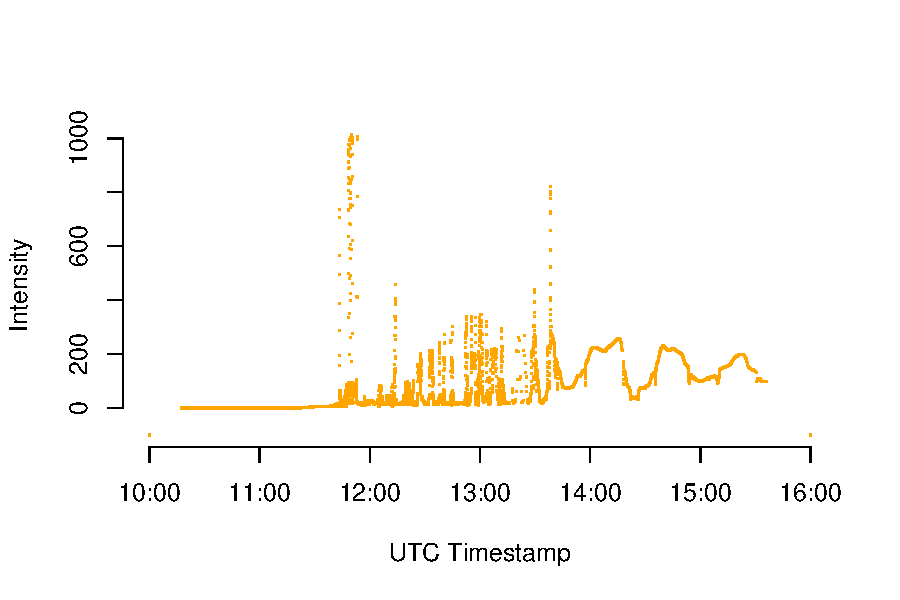
\includegraphics[width=8cm]{figures/photo_3.pdf}}
\hfill
\caption{Photodiode data from the flight.}
\label{fig:photodiodes}
\end{figure}


\subsection{Organic Solar Cell Results}
\label{sec:Solar-Cell-Results}

This is the solar cell results.
